\subsubsection{Exercise} 

\paragraph{Minimum phase case}

Figure \ref{steprepmin} shows the step response from one input at a time.

\begin{figure}[h!t]
        \centering
        \begin{subfigure}[b]{0.45\columnwidth}
                \includegraphics[width=\columnwidth]{fig/steprepmin75_0.eps}
                \caption{$u_1 = 75\%, u_2 = 0\%$}
        \end{subfigure}
        \begin{subfigure}[b]{0.45\columnwidth}
                \includegraphics[width=\columnwidth]{fig/steprepmin0_75.eps}
                \caption{$u_1 = 0\%, u_2 = 75\%$}
        \end{subfigure}
        \caption{Step response from one input at a time \\ for the minimum phase case} 
        \label{steprepmin}
\end{figure}

\paragraph{Non-minimum phase case} 

Figure \ref{steprepnonmin} shows the step response from one input at a time.

\begin{figure}[h!t]
        \centering
        \begin{subfigure}[b]{0.45\columnwidth}
                \includegraphics[width=\columnwidth]{fig/steprepnonmin0_75.eps}
                \caption{$u_1 = 75\%, u_2 = 0\%$}
        \end{subfigure}
        \begin{subfigure}[b]{0.45\columnwidth}
                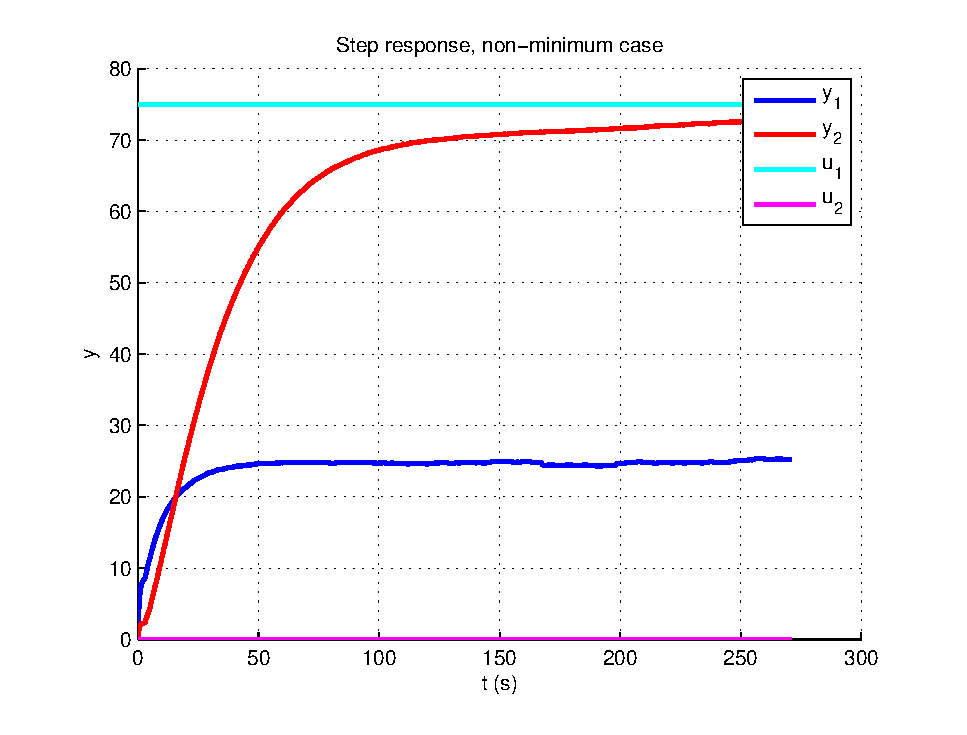
\includegraphics[width=\columnwidth]{fig/steprepnonmin75_0.eps}
                \caption{$u_1 = 0\%, u_2 = 75\%$}
        \end{subfigure}
        \caption{Step response from one input at a time \\ for the non-minimum phase case} 
        \label{steprepnonmin}
\end{figure}

